\section{Verwendung und Umfeld des JHelioviewers}
Wie der Name bereits verrät ist JHelioviewer eine Applikation,  die zur Analyse von Sonnendaten verwendet wird. Es wird international zur Sonnenforschung eingesetzt und wird von der FHNW zusammen mit der ESA entwickelt. Momentan ist eine neue Version des JHelioviewer in Entwicklung, welche die Sonne im dreidimensionalen Raum darstellt. Ein Feature von JHelioviewer ist die Magnetfeldlinien darzustellen und zu animieren, die Abbildung \ref{einleitung::feldlinien} zeigt die Visualisierung.
\begin{figure}[!htbp]
\center
	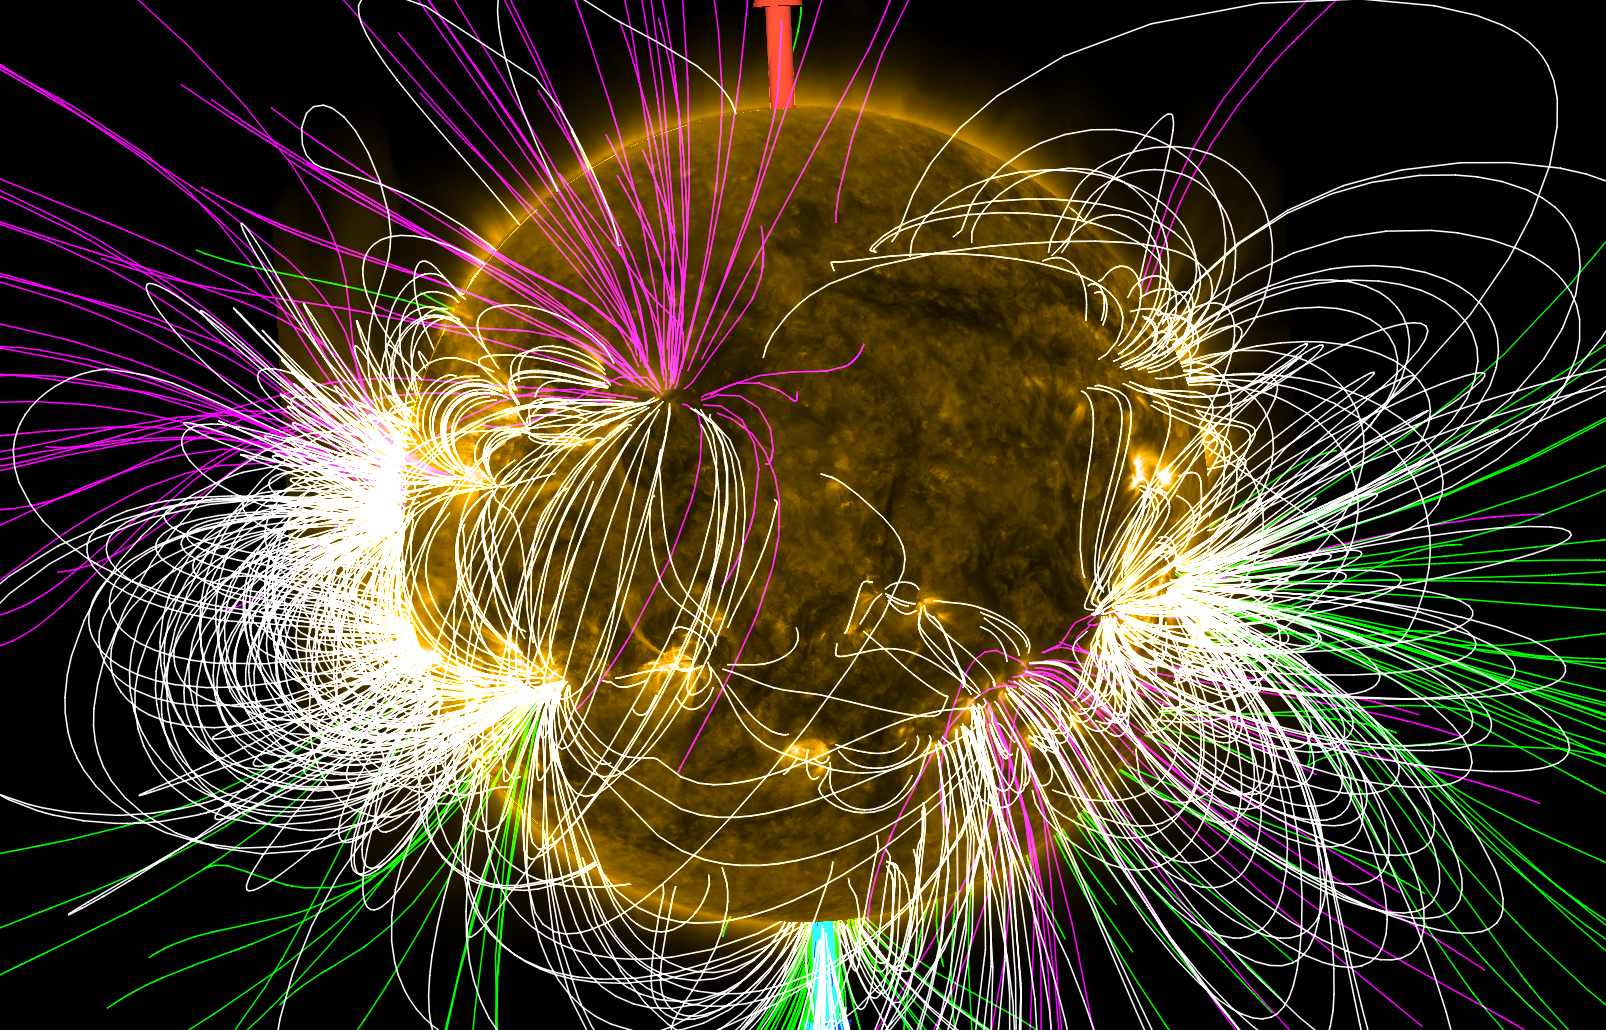
\includegraphics[scale=0.5]{./pictures/fieldLines.png}
	\caption{Visualisierung der Feldlinien im JHelioviewer}
	\label{einleitung::feldlinien}
\end{figure}
Es wird zwischen drei Feldlinien Unterschieden: Linien, die auf der Sonne starten und wieder auf der Sonne landen, auf der Sonne starten und ins Weltall führen oder vom Weltall auf der Sonne landen. Die weissen Feldlinien repräsentieren ''Sonne zu Sonne´´, die Grünen ''Sonne zu Weltall´´ und die Violetten ''Weltall zu Sonne´´. Die Feldlinien sind, allgemein Betrachtet, eine grosse Menge an Punkten, welche ein Server bereitstellt. Die Abbildung \ref{einleitung::aufbau} visualisiert den Datenfluss.
\begin{figure}[!htbp]
\center
	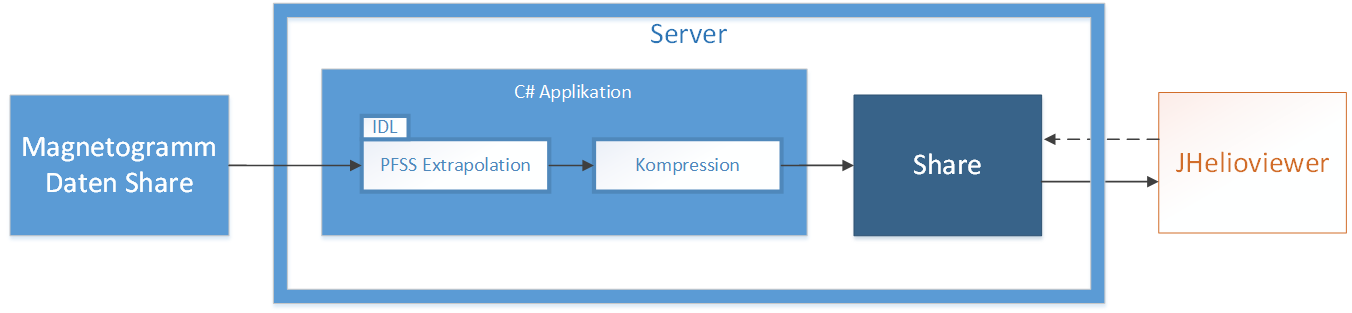
\includegraphics[scale=0.5]{./pictures/server.png}
	\caption{Aufbau und Datenfluss des Servers}
	\label{einleitung::aufbau}
\end{figure}
In regelmässigen Abständen sucht der Server nach neuen Oberflächen-Magnetogramm-Daten der Satelliten. Alle sechs Stunden wird die Oberfläche der Sonne neu gemessen.Daraus werden mittels Potential Field Source Surface (PFSS) Extrapolation die Feldlinien zu diesem Zeitpunkt errechnet. Danach führt der Server eine verlustlose Kompression durch und stellt die Daten auf einem öffentlichen Share dem JHelioviewer zur Verfügung. Der JHelioviewer lädt dann zur Laufzeit die Feldlinien, die er benötigt. 

Zukunft soll eine Feldlinienanimation angeboten werden, nicht nur alle 6 stunden sondern jede halbe Stunde.

\subsection{Datenmenge ist zu gross für die Datenübertragung}
Die Feldlinien der Sonne zu einem Zeitpunkt bringen etwa 1.3 MiBytes auf die Waage. 

Mit einer vernünftigen Bandbreite ist das flüssige Abspielen der Animation deshalb nicht möglich. Ziel ist es eine Kompression zu entwickeln, welche eine flüssige Animation erlaubt.\\[\baselineskip]
Im Vorfeld möglichst verlustfrei
Neu verlustbehaftet

Ziel ist es die Feldlinien verlustbehaftet zu komprimieren, sodass JHelioviewer eine möglichst flüsssige Animation anbieten kann. Die Komprimierung soll serverseitig mittels C\# umgesetzt werden während der JHelioviewer mit der Dekomprimierung ausgestattet wird.\\[\baselineskip] 
Verlustbehaftet, metriken!!

 